\documentclass[onecolumn, letterpaper, 12pt]{report}

% insert any packages, environments, counters, etc here
\usepackage{graphicx}
\usepackage{hyperref}

\begin{document}
%insert document contents here

\section{Intro}

Conv Nets are a specialized kind of neural network for processing data that has a known, grid like topology. Examples include time series data, which can be thought of as a 1D grid takings samples at regular time intervals, and image data which can be thought of as a 2D grid of pixels. 

The name convolutional neural network implies that the network employs a mathematical operation called a \textbf{convolution}. CNNs use convolution in place of general matrix multiplication in at least one of their layers. 

\section{The Convolution Operation}

The convolution is an operation on two functions of a real valued argument. Suppose we are tracking the location of a spaceship with a laser sensor. The laser provides a single output $x(t)$
, the position of the space ship at time $t$. Both $x$ and $t$ are real valued. 

Now suppose our laser sensor is noisy. To obtain a less noisy estimate of the ships position, we would like to average together several measurements. More recent measurements are more relevant, so we will want to give a weighted average with more weight to recent measurements. We can do this by applying a weighting function $w(a)$ where $a$ is the age of the measurement. 

If we apply such a weighted average operation at every moment, we obtain a new function $s$ providing a smoothed estimate of the position of the spaceship 

\begin{center}
  $s(t) = \int x(a) w(t - a) da$
\end{center}

This operation is called a convolution and is typically denoted with an asterisk

\begin{center}
  $s(t) = (x * w)(t) $
\end{center}


In our example, $w$ needs to be a valid probability distribution. In convolutional network terminology, the first argument ($x$) to the convolution is often referred to as the \textbf{input} and the second argument ($w$) is known as the \textbf{kernel}. The output is sometimes referred to as the \textbf{feature map}.

For a discrete convolution, we can assume that $t \in N$
. Then we can define the discrete convolution as 


\begin{center}
  $s(t) = (x * w)(t) = \sum\limits_{a = -\infty}^{\infty} x(a)w(t - a)$
\end{center}

In ml applications, the input is generally a multidimensional array of data and the kernel is usually a multidimensional array of parameters that are adapted by the learning algorithm. 

We often use convolutions over more than one axis at a time. For example, if we use a two dimensional image $I$ as our input, we also want to use a two dimensional kernel $K$: 

\begin{center}
  $s(i, j) = (I * K)(i, j) = \sum\limits_m \sum\limits_nI(m,n) K(i-m, j-n)$
\end{center}

Convolution is commutative, so equivalently we could write 

\begin{center}
  $s(i, j) = (I * K)(i, j) = \sum\limits_m \sum\limits_nI(i-m,j-n) K(m, n)$  
\end{center}

While the commutativity of convolutions is useful for writing proofs, in practice neural network libraries often implement a related function called \textbf{cross-correlation}, which is the same as convolution but without flipping the kernel: 

\begin{center}
  $s(i, j) = (I * K)(i, j) = \sum\limits_m \sum\limits_nI(i+m,j+n) K(m, n)$
\end{center}

Discrete convolution can be viewed as multiplication by a matrix. The matrix has several entries constrained to be equal to other entries. For example, for univariate discrete convolution, each row of the matrix is constrained to be equal to the row above shifted by one element. This is known as a \textbf{Toeplitz matrix}. In two dimensions, a \textbf{doubly block circulant matrix} corresponds to convolution. 

In addition to these constraints, convolution usually cooresponds to a very sparse matrix. This is because the kernel is usually much smaller than the input image. Any neural network algorithm that works with matrix multiplication and does not depend on specific properties of the matrix structure should work with convolution without requiring further changes to the network. 

\begin{figure}[h]
  \centering
  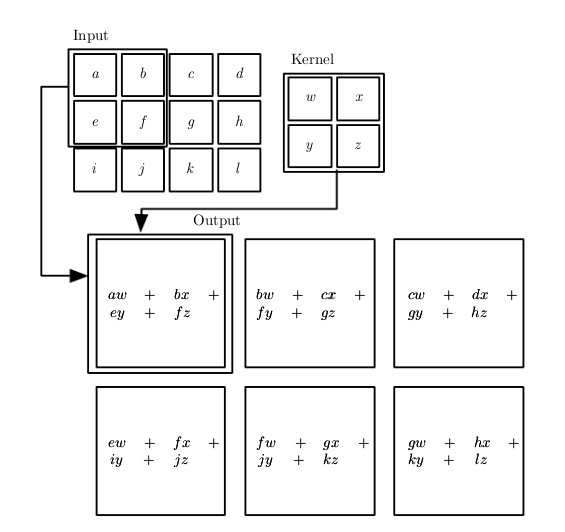
\includegraphics[width=0.7\textwidth]{conv_2d.png}
  \caption{2-D convolution without kernel flipping}
\end{figure}

\section{Motivation}

Convolution leverages three important ideas that can help improve a machine learning system: 

\begin{enumerate}
\item sparse interactions
\item parameter sharing
\item equivariant representations
\end{enumerate}

\subsection{sparse interactions}

Traditional neural networks layers use matrix multiplication by a matrix of parameters with a separate parameter describing the interaction between each input unit and each output unit. This means that each input unit interacts with each output unit.

Convolutional neural networks in contrast typically have \textbf{sparse interactions} (also referred to as sparse connectivity or sparse weights). This is accomplished by making the kernel smaller than the input. When processing an image, there may be thousands or millions of pixels, but we can detect small meaningful features such as edges with kernels that only occupy tens of pixels. This means we can store fewer parameters, reducing the space and time requirements and improving statistical efficiency. 

\begin{figure}[h]
  \centering
  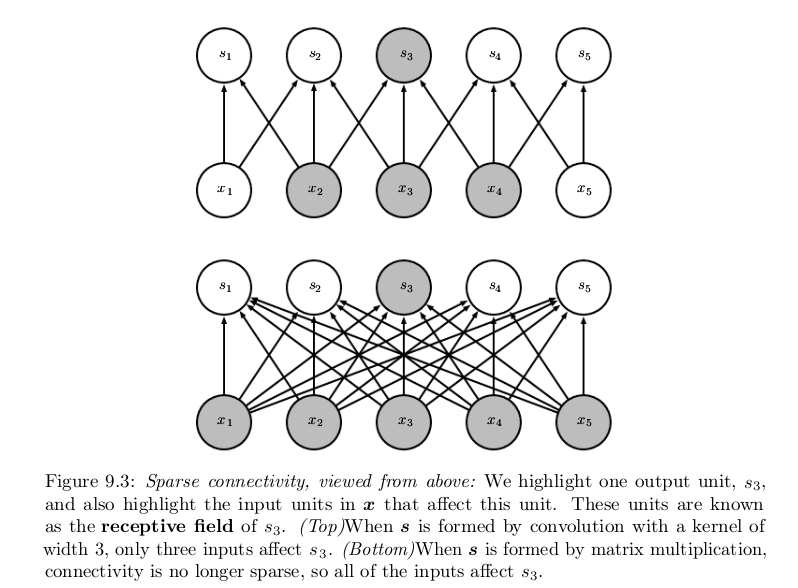
\includegraphics[width=0.7\textwidth]{sparse_connectivity.png}
\end{figure}

\subsection{parameter sharing}

\textbf{Parameter sharing} refers to using the same parameter for more than one function in a model. In a traditional network, we have \textbf{tied weights}. This means that the value of a weight applied to one input is tied to the value of a weight applied elsewhere. 

In a conv net, each member of the kernel is used at every position of the input (except perhaps the boundary pixels, depending on the design decisions). The parameter sharing used by the convolution operation means that rather than learning a separate set of parameters for every location, we can learn only one set. Convolution is thus dramatically more efficient than dense matrix multiplicationin terms of the memory requirements and statistical efficiency. 

\begin{figure}[h]
  \centering
  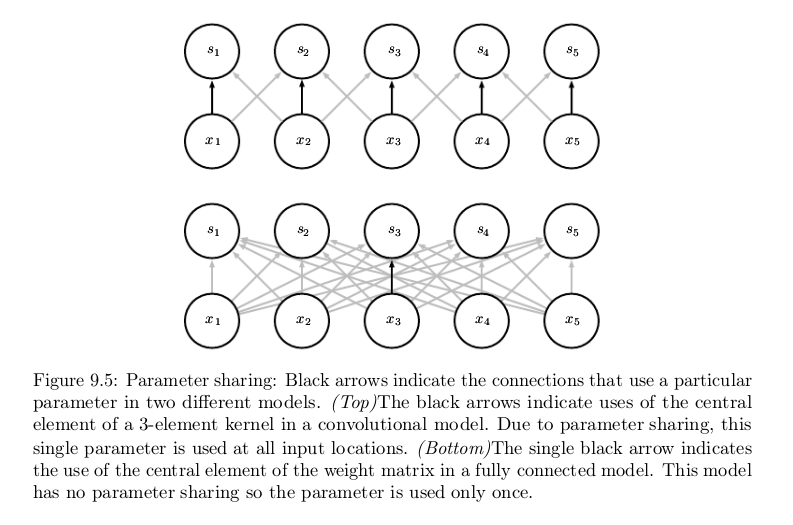
\includegraphics[width=0.7\textwidth]{param_sharing.png}
\end{figure}

\subsection{equivariance}

In the case of convolution, the particular form of parameter sharing causes the layer to have a property called \textbf{equivariance} to translation. To say a function is equivariant means that if the input changes, the output changes in the same way. Specifically, a function $f(x)$ is equivariant to a function $g$ if $f(g(x)) = g(f(x))$. In the case of convolution, if we let $g$ be any function that translates the input, i.e. shifts it, then the convolution function is equivariant to $g$. 

Convolution is not naturally equivariant to some other transformations, such as changes in the scale or rotation of an image. Other mechanisms are necessary for handling these kinds of transformations. 

\section{Pooling}

A typical layer of a convolutional neural network consists of three stages: 

1. The layer performs several convolutions in parallel to produce a set of linear activations.
2. Each linear activation is run through a nonlinear activation function, such as ReLU
3. This stage is sometimes called the \textbf{detector} stage. We use a \textbf{pooling function} to modify the output of the layer further. 

A pooling function replaces the output of the net at a certain location with a summary statistic of the nearby outputs. For example, max pooling returns the maximum output within a rectangular neighborhood. Other popular pooling functions include the average, the $L^2$ norm, or a weighted average based on the distance from the central pixel. 

\begin{figure}[h]
  \centering
  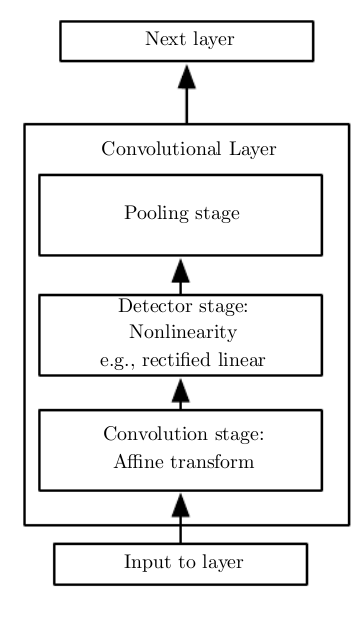
\includegraphics[width=0.3\textwidth]{conv_layer.png}
\end{figure}

In all cases, pooling helps to make the representation become approximately invariant to small translations of the input. Invariance to local translation can be a very useful property if we care more about whether some feature is present than exactly where it is. The use of pooling can be viewed as adding an infinitely strong prior that the function the layer learns must be invariant to small translations. When this assumption is correct, it can greatly improve the efficiency of the network. 

For many tasks, pooling is essential for handling inputs of varying size. For example, if we want to classify images of variable size, the input to the classification layer must have a fixed size. This is usually accomplished by varying the size of an offset between pooling regions so that the classification layer always receives the same number of summary statistics regardless of the input size. 

Some theoretical work gives guidance on which kinds of pooling to use in various situations (Boureau et al, 2010):

\begin{quote}
\href{https://www.di.ens.fr/willow/pdfs/icml2010b.pdf}{A Theoretical Analysis of Feature Pooling in Visual Recognition}  
\end{quote}

\begin{quote}
  Many modern visual recognition algorithms incorporate a step of
  spatial ‘pooling’, where the outputs of several nearby feature
  detectors are combined into a local or global ‘bag of features’, in
  a way that preserves task-related information while removing
  irrelevant details. Pooling is used to achieve invariance to image
  transformations, more compact representations, and better robustness
  to noise and clutter. Several papers have shown that the details of
  the pooling operation can greatly influence the performance, but
  studies have so far been purely empirical. In this paper, we show
  that the reasons underlying the performance of various pooling
  methods are obscured by several confounding factors, such as the
  link between the sample cardinality in a spatial pool and the
  resolution at which low-level features have been extracted. We
  provide a detailed theoretical analysis of max pooling and average
  pooling, and give extensive empirical comparisons for object
  recognition tasks.
\end{quote}

It is also possible to dynamically pool features together, for example, by running a clustering algorithm on the locations of interesting features (Boureau et al, 2011). This approach yields a different set of pooling regions for each image. 

\begin{quote}
\href{https://www.di.ens.fr/~fbach/boureau-iccv-11.pdf}{Ask the locals: multi-way local pooling for image recognition}
\end{quote}

\begin{quote}
  Invariant representations in object recognition systems are
  generally obtained by pooling feature vectors over spatially local
  neighborhoods. But pooling is not local in the feature vector space,
  so that widely dissimilar features may be pooled together if they
  are in nearby locations. Recent approaches rely on sophisticated
  encoding methods and more specialized codebooks (or dictionaries),
  e.g., learned on subsets of descriptors which are close in feature
  space, to circumvent this problem. In this work, we argue that a
  common trait found in much recent work in image recognition or
  retrieval is that it leverages locality in feature space on top of
  purely spatial locality. We propose to apply this idea in its
  simplest form to an object recognition system based on the spatial
  pyramid framework, to increase the performance of small dictionaries
  with very little added engineering. Stateof-the-art results on
  several object recognition benchmarks show the promise of this
  approach.
\end{quote}

Another approach is to learn a single pooling structure that is then applied to all images (Jia et al, 2012)

\begin{quote}
  \href{http://www.icsi.berkeley.edu/pubs/vision/beyondspatial12.pdf}{Beyond Spartial Pyramids: Receptive Field Learning for Pooled Image Features}
\end{quote}

\begin{quote}
  In this paper we examine the effect of receptive field designs on
  classification accuracy in the commonly adopted pipeline of image
  classification. While existing algorithms usually use manually
  defined spatial regions for pooling, we show that learning more
  adaptive receptive fields increases performance even with a
  significantly smaller codebook size at the coding layer. To learn
  the optimal pooling parameters, we adopt the idea of
  over-completeness by starting with a large number of receptive field
  candidates, and train a classifier with structured sparsity to only
  use a sparse subset of all the features. An efficient algorithm
  based on incremental feature selection and retraining is proposed
  for fast learning. With this method, we achieve the best published
  performance on the CIFAR-10 dataset, using a much lower dimensional
  feature space than previous methods.
\end{quote}

\section{Convolution and Pooling as an Infinitely Strong Prior}

Priors can be considered weak or strong depending on how concentrated the probability density in the prior is. A weak prior is a distribution with high entropy, such as a Gaussian with high variance. Such a prior allows the data to move the parameters more or less freely. A strong prior has very low entropy, such as a Gaussian with low variance. Such a prior plays an active role in determining where the parameters end up. An infinitely strong prior places zero probability on some parameters and says that these prarameter values are completely forbidden, regardless of any support from the data. 

We can imagine a convolutional net as being similar to a fully connected net, but with an infinitely strong prior over its weights. This infinitely strong prior says that the weights for one hidden unit must be identical to the weights of its neighbor, but shifted in space. 

\end{document}
